%-------------------------------------------------------------------------------
%-------------------------------------------------------------------------------
%-------------------------------------------------------------------------------
\chapter{Vagues et structures}
%-------------------------------------------------------------------------------
%-------------------------------------------------------------------------------
%-------------------------------------------------------------------------------

Ce sujet est une adaptation du sujet des Mines 2020
%-------------------------------------------------------------------------------
\begin{figure}[ht]
\begin{center}
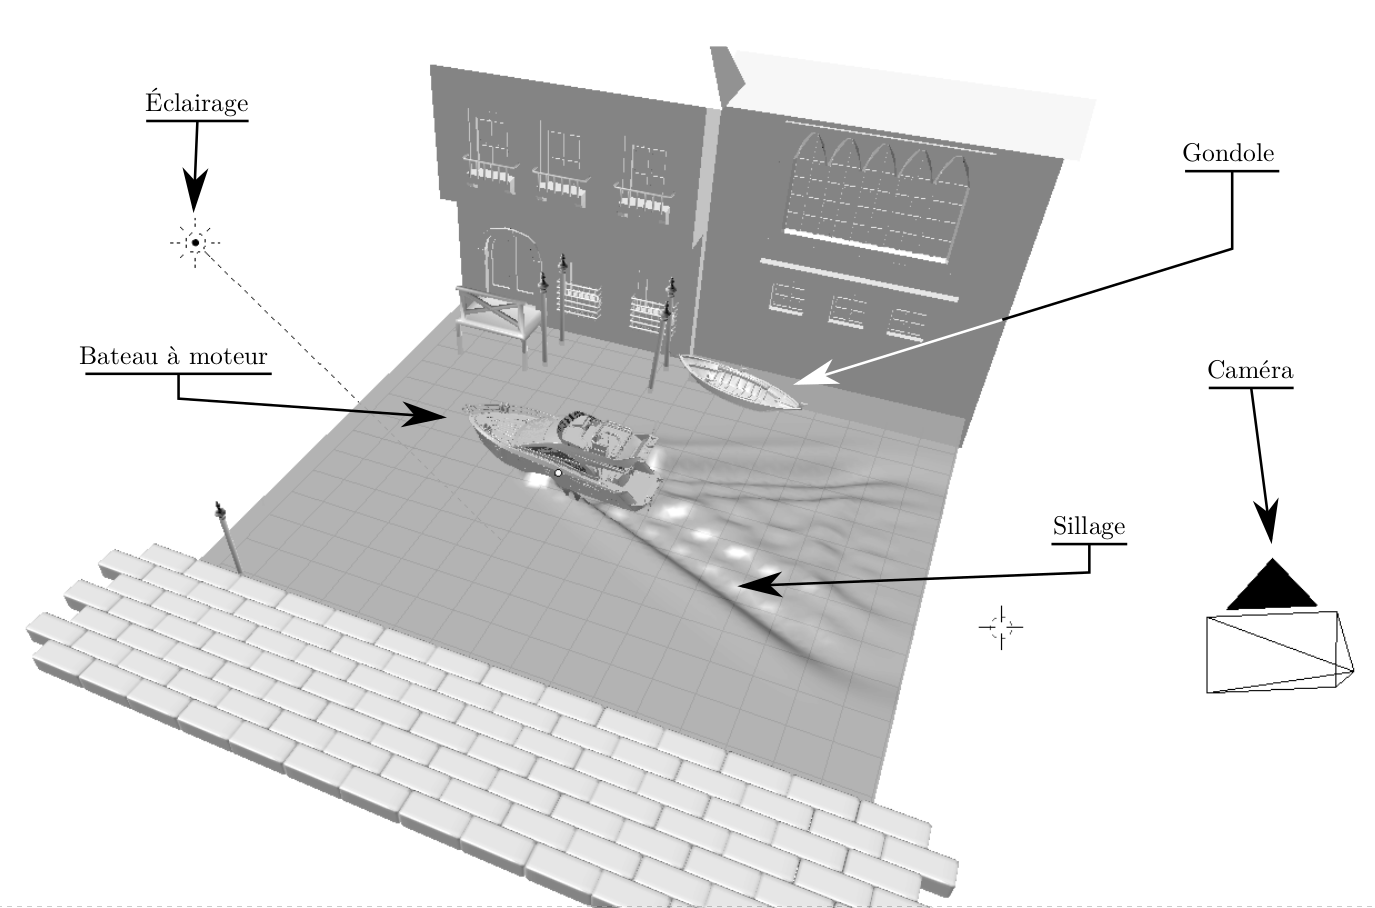
\includegraphics[width=\linewidth]{Mines_2020_scene}
\caption{Présentation de la scène étudiée}
\end{center}
\end{figure}
%-------------------------------------------------------------------------------
\newpage
%-------------------------------------------------------------------------------
%-------------------------------------------------------------------------------
%-------------------------------------------------------------------------------
\subsection*{Préambule} 
%-------------------------------------------------------------------------------
%-------------------------------------------------------------------------------
Dans une production cinématographique en images de synthèse, les images sont crées une à une pour
donner l’illusion du mouvement (sur le principe du dessin animé). Pour satisfaire les spectateurs,
il est efficace de réaliser des images conformes aux équations de la physique.

Le sujet aborde la réalisation d’une scène montrant un bateau à moteur traversant un canal, créant
un sillage à la surface de l’eau, et faisant osciller une gondole amarrée à proximité. 

Il n’est pas nécessaire d’avoir réussi à écrire le code d’une fonction pour pouvoir s’en servir dans une autre question.

\medskip

Partout où cela est nécessaire, les variables sont considérées être exprimées dans les unités SI. 

Le repère $\bigl(O, \vec e_x, \vec e_y, \vec e_z\bigr)$ servant de référentiel est fixe par rapport au décor.
%-------------------------------------------------------------------------------
%-------------------------------------------------------------------------------
\subsection*{Modèle de facettes} 
%-------------------------------------------------------------------------------
%-------------------------------------------------------------------------------
La scène contient plusieurs objets géométriques tri-dimensionnels (3D). Chaque objet géométrique
est représenté de manière numérique par un maillage. 
%-------------------------------------------------------------------------------
\begin{figure}[ht]
\begin{center}
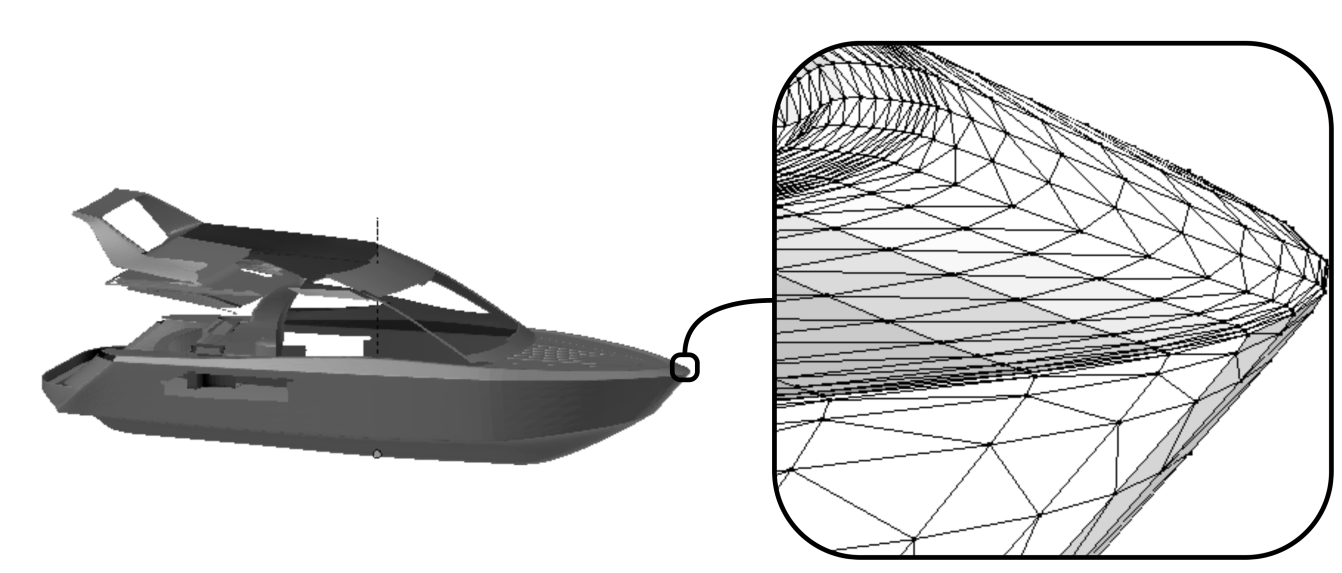
\includegraphics[width=\linewidth]{Mines_2020_bateau}
\caption{Un exemple de maillage : la coque d'un bateau}
\end{center}
\end{figure}
%-------------------------------------------------------------------------------

%-------------------------------------------------------------------------------
\begin{minipage}{0.55\linewidth}
On définit les termes suivants :

\begin{description}
\item[Maillage] : ensemble des facettes qui constituent la géométrie d’un objet. Un maillage sera
représenté par une liste de facettes.
\item[Facette] : polygone élémentaire qui constitue une partie de la surface d’un objet. Ici, toutes les
facettes seront des triangles. Une facette sera représentée par une liste ordonnée de 3 sommets.
\item[Sommet] : point délimitant une facette. Il peut être commun à une ou plusieurs facettes. Tout
point sera représenté par son vecteur position de coordonnées $(x,y,z)$. 
\end{description}

La figure ci-contre représente un exemple de maillage simple (tétraèdre), 

composé de 4 facettes (notées $S_1$ à $S_4$) 

et de 4 sommets (notés $A$ à $D$) 

avec $AB = AD = AC = 1$. 
\end{minipage}
%-------------------------------------------------------------------------------
\begin{minipage}{0.45\linewidth}
\begin{center}
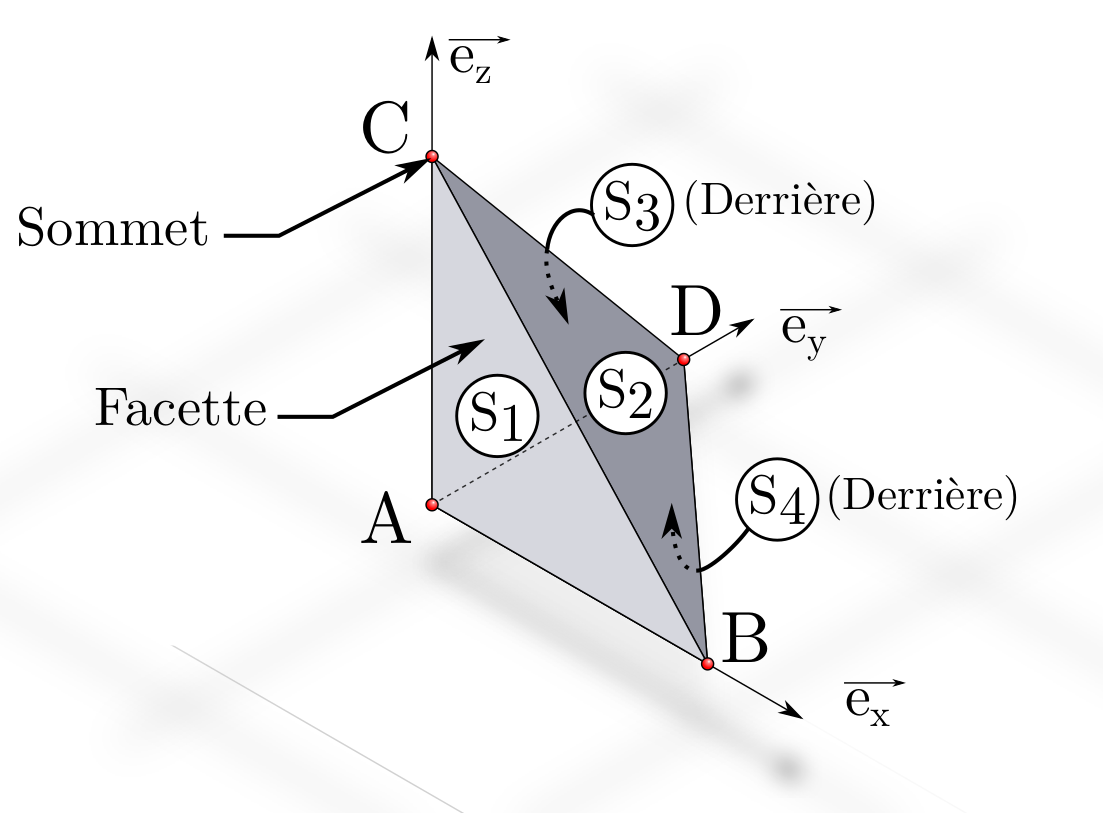
\includegraphics[width=1.2\linewidth]{Mines_2020_tetra}
\end{center}
\end{minipage}
%-------------------------------------------------------------------------------
\newpage
%-------------------------------------------------------------------------------
%-------------------------------------------------------------------------------
\subsection*{Numpy} 
%-------------------------------------------------------------------------------
%-------------------------------------------------------------------------------
On utilisera les vecteurs (\type{array}) du module \type{numpy}.
\begin{lstlisting}
import numpy as np
\end{lstlisting}
Par exemple, un vecteur dont les coordonnées sont $x = 2$, $y = 3$ et $z = 1,5$ sera defini par :
\begin{lstlisting}
V = np.array([2.0, 3.0, 1.5])
\end{lstlisting}
On rappelle qu'il est affiché par \type{array([2.0, 3.0, 1.5])}.

\medskip


\begin{itemize}
    \item Un sommet point est représenté par un vecteur \type{numpy}, $A$ est assimilé à $\overrightarrow{OA}$.
    \item Si \type{a} et \type{b} représentent les points $A$ et $B$, le vecteur $\overrightarrow{AB}$ est déterminé par \type{b - a}.
    \item On peut additionner les vecteurs \type{numpy} de même taille.
    \item On peut multiplier un vecteur par un scalaire.
    \item Le produit scalaire $\vec u.\vec v$ de deux vecteurs représentés par les vecteurs \type{numpy} \type{u} et \type{v} est obtenu par \type{np.dot(u, v)}.
    \item Le produit vectoriel $\vec u \wedge \vec v$ est calculé par \type{np.cross(u, v)}.
\end{itemize}
%-------------------------------------------------------------------------------
%-------------------------------------------------------------------------------
\subsection*{Représentation Python} 
%-------------------------------------------------------------------------------
%-------------------------------------------------------------------------------
\begin{itemize}
\item Une facette triangulaire est représentée par la liste de ses 3 sommets.
\item Un maillage est représenté par la liste de ses facettes.
\end{itemize}

Par exemple, le tétraèdre ci-dessus sera défini par la variable \type{maillage\_tetra}
\begin{lstlisting}
A = np.array([0.0, 0.0, 0.0])
B = np.array([1.0, 0.0, 0.0])
C = np.array([0.0, 0.0, 1.0])
D = np.array([0.0, 1.0, 0.0])

maillage-tetra = [[A, B, C], [A, D, C], [A, B, D], [B, D, C]]
\end{lstlisting}
%-------------------------------------------------------------------------------
%-------------------------------------------------------------------------------
%-------------------------------------------------------------------------------
\section{Objets de la scène} 
%-------------------------------------------------------------------------------
%-------------------------------------------------------------------------------
%-------------------------------------------------------------------------------
\subsection{Travail sur les facettes} 
%-------------------------------------------------------------------------------
%-------------------------------------------------------------------------------
\begin{Exercise}\it 
À partir de la variable \type{maillage\_tetra}, écrire une expression Python permettant de récupérer la coordonnée $y$ du premier sommet de la première facette.
\end{Exercise}
%-------------------------------------------------------------------------------
\begin{Answer}
\begin{lstlisting}
maillage_tetra[0][0][1]
\end{lstlisting}
\end{Answer}
%-------------------------------------------------------------------------------
%-------------------------------------------------------------------------------
\begin{Exercise}\it 
À quel élément, sur la figure de la page 2, correspond \type{maillage\_tetra[1]} ?
\end{Exercise}
%-------------------------------------------------------------------------------
\begin{Answer}
La facette $(A, D,C)$ correspond à la facette $S_3$.
\end{Answer}
%-------------------------------------------------------------------------------
%-------------------------------------------------------------------------------
\medskip

On considère la fonction suivante, prenant un vecteur comme paramètre
\begin{lstlisting}
def mystere1 (V):
    x, y, z = V
    return (x**2 + y**2 + z**2)**0.5
\end{lstlisting}
%-------------------------------------------------------------------------------
%-------------------------------------------------------------------------------
\begin{Exercise}\it 
Que fait la fonction \type{mystere1} ?

Proposer un nom plus adapté pour la fonction ; on pourra utiliser la fonction avec ce nouveau nom.
\end{Exercise}
%-------------------------------------------------------------------------------
\begin{Answer}

La fonction calcule la norme du vecteur $V$. On pouvait l'appeler \type{norme}.
\end{Answer}
%-------------------------------------------------------------------------------
%-------------------------------------------------------------------------------
\begin{Exercise}\it 
Écrire une fonction \type{barycentre(F)}, prenant comme argument une facette \type{F} (une liste de 3 sommets) et renvoyant le barycentre de la facette, c'est-à-dire le point dont les coordonnées sont les moyennes des coordonnées des sommets.
\end{Exercise}
%-------------------------------------------------------------------------------
\begin{Answer}
\begin{lstlisting}
def barycentre(F):
    A, B, C = F
    return (A + B + C)/3
\end{lstlisting}
\end{Answer}
%-------------------------------------------------------------------------------
%-------------------------------------------------------------------------------

\medskip

On admet que l'aire d'un triangle $(ABC)$ est calculée par ${\cal A}(ABC)=\bigl\|\overrightarrow{AB} \wedge \overrightarrow{AC}\bigr\|$.
%-------------------------------------------------------------------------------
%-------------------------------------------------------------------------------
\begin{Exercise}\it 
Écrire une fonction \type{aire(F)}, prenant comme argument une facette \type{F} et renvoyant son aire.
\end{Exercise}
%-------------------------------------------------------------------------------
\begin{Answer}
\begin{lstlisting}
def aire(F):
    A, B, C = F
    N = np.cross(B-A, C-A)
    return norme(N)
\end{lstlisting}
\end{Answer}
%-------------------------------------------------------------------------------
%-------------------------------------------------------------------------------

\medskip

Le {\bf vecteur unitaire normal} d'une facette \type{F = [A, B, C]} d'aire non nulle est calculé  par  \[ \vec n =\frac{\overrightarrow{AB} \wedge \overrightarrow{AC}}{\bigl\|\overrightarrow{AB} \wedge \overrightarrow{AC}\bigr\|}\]
%-------------------------------------------------------------------------------
%-------------------------------------------------------------------------------
\begin{Exercise}\it 
Écrire une fonction \type{normal(F)}, prenant comme argument une facette \type{F} et renvoyant le vecteur unitaire normal.
\end{Exercise}
%-------------------------------------------------------------------------------
\begin{Answer}
\begin{lstlisting}
def normal(F):
    A, B, C = F
    N = np.cross(B-A, C-A)
    return (1/norme(N))*N
\end{lstlisting}
\end{Answer}
%-------------------------------------------------------------------------------
%-------------------------------------------------------------------------------
\subsection{Liste des sommets} 
%-------------------------------------------------------------------------------
%-------------------------------------------------------------------------------
Compte tenu de la représentation limitée des nombres réels en machine, deux sommets $S_1$ et $S_2$ supposés être au même endroit peuvent avoir des coordonnées légèrement différentes. 
%-------------------------------------------------------------------------------
%-------------------------------------------------------------------------------
\begin{Exercise}\it 
Proposer une fonction \type{sont\_proches(S1, S2, epsilon)}, prenant comme arguments deux sommets \type{S1} et \type{S2} et un flottant strictement positif \type{epsilon}, et qui renvoie \type{True} si $S_1$ et $S_2$ sont proches (i.e. si leur distance au sens de la norme Euclidienne est inférieure à $\varepsilon$) et \type{False} sinon.
\end{Exercise}
%-------------------------------------------------------------------------------
\begin{Answer}
\begin{lstlisting}
def sont_proches(S1, S2, epsilon):
    distance = norme(S2 - S1)
    return distance < epsilon
\end{lstlisting}
\end{Answer}
%-------------------------------------------------------------------------------
%-------------------------------------------------------------------------------

\medskip
Soient les fonctions suivantes :
\begin{lstlisting}
def mystere2(S1, L):
    for S2 in L :
        if sont_proches (S1, S2, 1e-7):
            return True
    return False
\end{lstlisting}

\begin{lstlisting}
def mystere3(maillage):
    res = []
    for facette in maillage:
        for sommet in facette:
             if not mystere2(sommet, res):
                 res.append(sommet)
    return res
\end{lstlisting}
%-------------------------------------------------------------------------------
%-------------------------------------------------------------------------------
\begin{Exercise}\it 
Sous quelle condition la fonction \type{mystere2} renvoie-t-elle \type{True} ?
\end{Exercise}
%-------------------------------------------------------------------------------
\begin{Answer}
La fonction \type{mystere2} renvoie \type{True}  si le sommet \type{S1} est proche de l'un des sommets de la liste \type{L}, avec une précision de $10^{-7}$.
\end{Answer}
%-------------------------------------------------------------------------------
%-------------------------------------------------------------------------------
\begin{Exercise}\it 
Donner (sans justification) ce que renvoie \type{mystere3(maillage\_tetra)}, où \type{maillage\_tetra} est la variable définie précédemment.
\end{Exercise}
%-------------------------------------------------------------------------------
\begin{Answer}
\type{mystere3(maillage\_tetra)} renvoie les sommets distincts à $10^{-7}$ près du maillage. Ici la fonction renvoie

\begin{lstlisting}
[array([0., 0., 0.]), array([0., 0., 1.]), 
 array([0., 1., 0.]), array([1., 0., 0.])]
\end{lstlisting}
\end{Answer}
%-------------------------------------------------------------------------------
%-------------------------------------------------------------------------------
\begin{Exercise}\it 
Pour une liste \type{L} de longueur $n$, discuter la complexité de la fonction \type{mystere2}. En déduire la complexité de \type{mystere3}, pour un maillage contenant $m$ facettes triangulaires. On distinguera le meilleur et le pire des cas.
\end{Exercise}
%-------------------------------------------------------------------------------
\begin{Answer}
La fonction \type{mystere2(S1, L)} fait un nombre constant d'instructions par passage dans la boucle.

Le meilleur cas est celui où \type{S1} est proche du premier élément de \type{L}, ce qui n'occasionne qu'un passage dans la boucle, d'où une complexité en ${\cal O}(1)$.

Au pire \type{S1} n'est proche d'aucun élément de la liste est la boucle est parcourue $n$ fois d'où une complexité en ${\cal O}(n)$.

\medskip

Pour la fonction  \type{mystere3(maillage)}, on applique  la fonction \type{mystere2(S, res)} pour tous les sommets du maillage, il y en a $3m$.

Dans le meilleur des cas, tous les sommets sont proches du premier et la complexité est alors proportionnelle à $m$ : ${\cal O}(m)$.


Dans le pire cas, aucun sommet n'est proche d'un autre sommet. La liste \type{res} est de longueur $k-1$ lors du traitement du $k$-ième sommet d'où une complexité majorée par 

$\displaystyle \sum_{k=1}^{3m} A.(k-1) = A\frac{3m(3m-1)}2 = 
{\cal O}(m^2)$.
\end{Answer}
% %-------------------------------------------------------------------------------
% %-------------------------------------------------------------------------------
% %-------------------------------------------------------------------------------
% \section{Génération de vagues} 
% %-------------------------------------------------------------------------------
% %-------------------------------------------------------------------------------
% %-------------------------------------------------------------------------------

% Le bateau à moteur qui traverse le canal génère des vagues (appelées {\bf sillage de Kelvin}). On ne
% dispose de formules analytiques décrivant ces ondes que dans des cas très simples, comme celui
% d’un bateau en translation rectiligne uniforme.

% Le calcul numérique permettant d’évaluer la forme de ces vagues étant coûteux, il est réalisé par
% un programme extérieur. Ce dernier génère l’état du plan d’eau à chaque image de la scène (25 par
% seconde).

% Pour chacune de ces images, on représente le plan d’eau par une grille régulière carrée, de taille
% $(m + 1) \times (m + 1)$. Chaque case $(i,j)$ de cette grille correspond à un sommet du maillage
% de la surface de l’eau, noté $n_{i,j}$, de coordonnées $(x_i ,y_j )$ (avec $(i,j) \in [\!| 0;m|\!]^2$).


% La hauteur (sur $\vec e_z$ de $n_{i,j}$ est notée $h_{i,j}$ . L’ensemble de tous les $h_{i,j}$ est stocké dans une liste de listes nommée \type{mat\_h}, telle que \type{mat\_h[i][j]} contiennent la valeur $h_{i,j}$.

% Le programme extérieur calcule ainsi \type{mat\_h} pour chaque nouvelle image. L’ensemble de toutes les
% valeurs de \type{mat\_h} est stocké dans une liste nommée \type{liste\_vagues}.

% La scène est composée de 350 images. Le plan d’eau est composé de $200 \times 200$ sommets. Chaque
% hauteur $h_{i,j}$ est un flottant codé sur 64 bits.

% %-------------------------------------------------------------------------------
% \begin{figure}[ht]
% \begin{center}
% 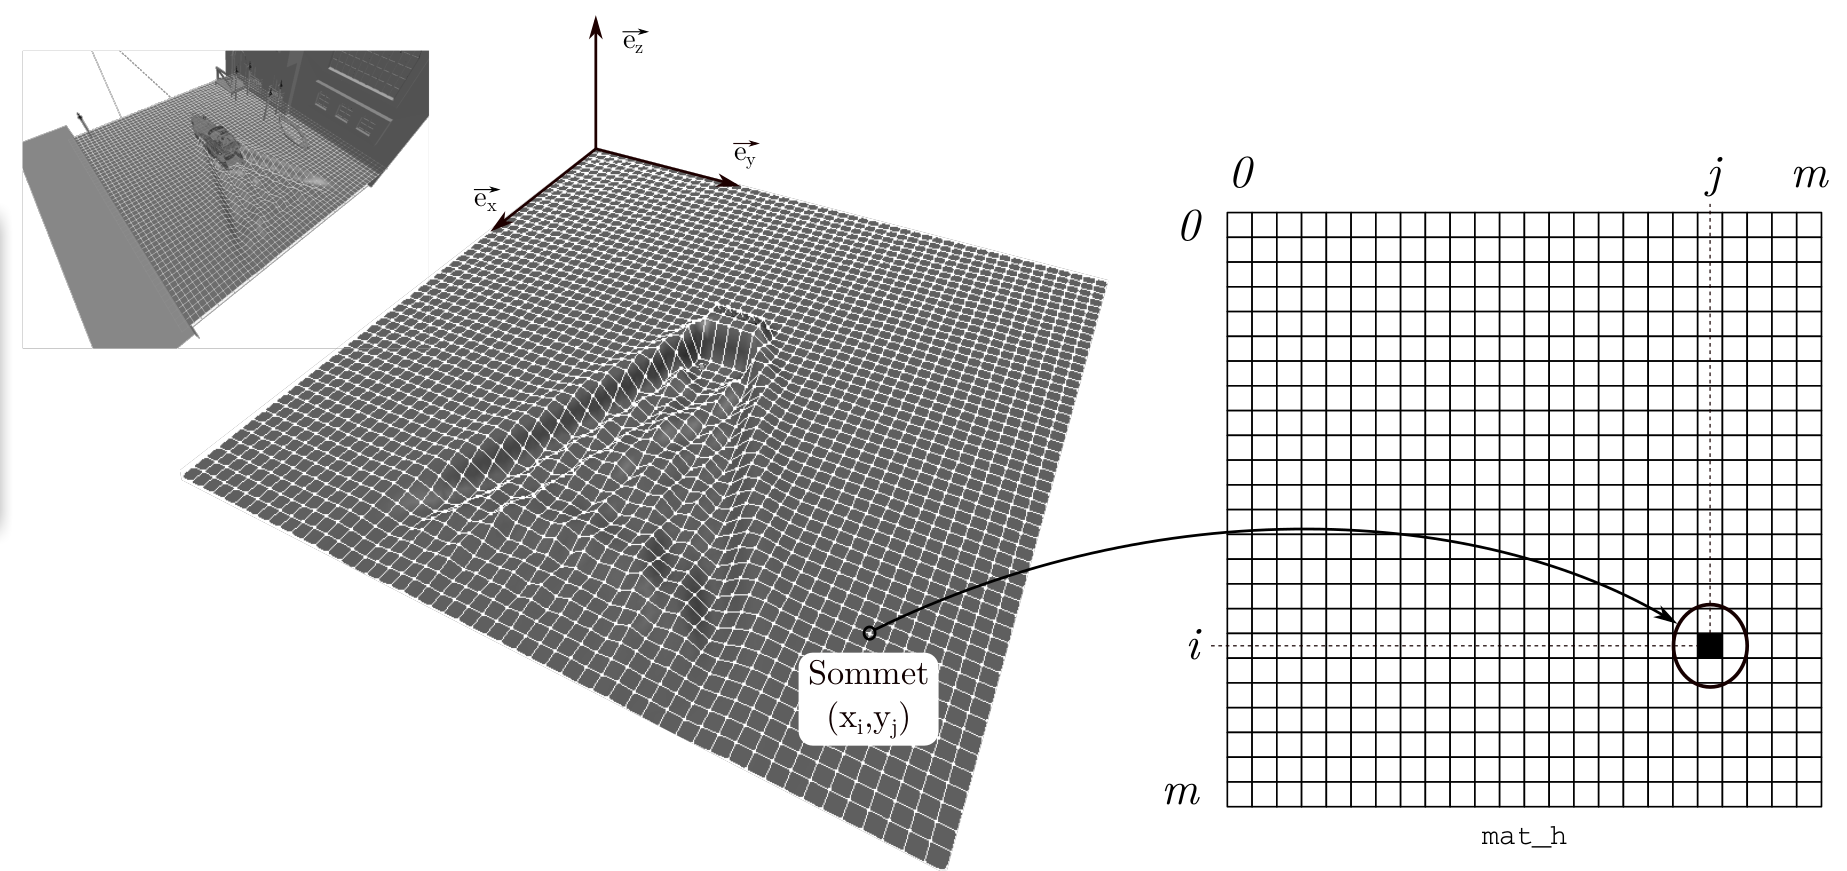
\includegraphics[width=\linewidth]{Mines_2020_vagues}
% \caption{Illustration du stockage de la hauteur d’eau dans un tableau}
% \end{center}
% \end{figure}
% %-------------------------------------------------------------------------------


% %-------------------------------------------------------------------------------
% %-------------------------------------------------------------------------------
% \begin{Exercise}\it 
% Quel est l’espace occupé en mémoire vive par l’ensemble des données en mega-octets ?
% % M o
% \end{Exercise}
% %-------------------------------------------------------------------------------
% \begin{Answer}
% \begin{lstlisting}

% \end{lstlisting}
% \end{Answer}
% %-------------------------------------------------------------------------------
% %-------------------------------------------------------------------------------

% \medskip

% On souhaite enregistrer le contenu de \type{liste\_vagues} dans un fichier afin de le transmettre au logiciel d’animation.
% %-------------------------------------------------------------------------------
% %-------------------------------------------------------------------------------
% \begin{Exercise}\it 
%  Écrire une fonction \type{mat2str(mat\_h} qui prend en argument une liste de listes et renvoie les données qu'elle contient sous forme d’une chaîne de caractères qui respecte le format suivant :
 
% $h_{0, 0}; h_{0, 1}; \cdots; h_{0, m}$

% $h_{1, 0}; h_{1, 1}; \cdots; h_{1, m}$

% $\quad \cdots$

% $h_{m, 0}; h_{m, 1}; \cdots; h_{m, m}$

% \end{Exercise}
% %-------------------------------------------------------------------------------
% \begin{Answer}
% \begin{lstlisting}

% \end{lstlisting}
% \end{Answer}
% %-------------------------------------------------------------------------------
% %-------------------------------------------------------------------------------
% On rappelle que le retour à la ligne est codé par le caractère "$\backslash n$".


% %-------------------------------------------------------------------------------
% %-------------------------------------------------------------------------------
% \begin{Exercise}\it 
% En s’appuyant sur mat2str, proposer un code Python qui permet de sauvegarder le contenu de \type{liste\_vagues} dans un fichier nommé {\sf fichier\_vagues.txt} (dans le répertoire courant), en séparant la représentation de chaque \type{mat\_h} par deux sauts de lignes consécutifs.
% \end{Exercise}
% %-------------------------------------------------------------------------------
% \begin{Answer}
% \begin{lstlisting}

% \end{lstlisting}
% \end{Answer}
% %-------------------------------------------------------------------------------
% %-------------------------------------------------------------------------------

% \medskip

% Le fichier texte obtenu est jugé trop volumineux. On décide de recourir à des matrices creuses. Dans ce qui suit on désigne par matrice creuse une matrice dont seuls la valeur et l’emplacement des éléments non-nuls (c’est-à-dire significativement éloignés de zéro) sont enregistrés. On propose d’utiliser le format de fichier nommé {\sf Coordinate Format} qui consiste à stocker :

% \begin{itemize}
%     \item une liste \type{I}, comportant les numéros de ligne de chaque élément non-nul,
%     \item une liste \type{J}, comportant les numéros de colonne de chaque élément non-nul,
%     \item une liste \type{N}, comportant la valeur de chaque élément non-nul.
% \end{itemize}

% Les valeurs d’une liste sont enregistrées sur une même ligne et séparées par des points-virgules. Chaque liste est séparée des autres par un retour à la ligne. On admet que les flottants sont écrits dans le fichier avec 15 caractères (tout compris).

% %-------------------------------------------------------------------------------
% %-------------------------------------------------------------------------------
% \begin{Exercise}\it 
% Après avoir défini judicieusement les types des éléments contenus dans \type{I}, \type{J} puis \type{N}, estimer la taille (en octets) que prendra une matrice ayant $p$ éléments non-nuls, au format {\sf Coordinate Format}, dans le fichier.
% \end{Exercise}
% %-------------------------------------------------------------------------------
% \begin{Answer}
% \begin{lstlisting}

% \end{lstlisting}
% \end{Answer}
% %-------------------------------------------------------------------------------
% %-------------------------------------------------------------------------------
% \begin{Exercise}\it 
% En déduire à partir de combien d’éléments non-nuls il devient moins avantageux d’enregistrer une matrice creuse qu'une matrice complète classique.
% \end{Exercise}
% %-------------------------------------------------------------------------------
% \begin{Answer}
% \begin{lstlisting}

% \end{lstlisting}
% \end{Answer}
% %-------------------------------------------------------------------------------
% %-------------------------------------------------------------------------------
% \begin{Exercise}\it 
% Proposer un code permettant de construire, pour un tableau \type{mat\_h} donné, les listes Python \type{I}, \type{J} et \type{N}. On considérera nulles les hauteurs inférieures à $10^{-3}$ (en valeur absolue).
% \end{Exercise}
% %-------------------------------------------------------------------------------
% \begin{Answer}
% \begin{lstlisting}

% \end{lstlisting}
% \end{Answer}
%-------------------------------------------------------------------------------
\newpage
%-------------------------------------------------------------------------------
%-------------------------------------------------------------------------------
\section{Mouvement de flottaison} 
%-------------------------------------------------------------------------------
%-------------------------------------------------------------------------------
%-------------------------------------------------------------------------------
La gondole amarrée sur le bord du canal perçoit les vagues générées par le bateau à moteur et effectue un mouvement pseudo-oscillant conséquence de sa flottaison. On étudie ici le mouvement de translation verticale de la gondole (on ne prendra en compte ni le tangage ni le roulis). On cherche à modéliser ce mouvement en calculant à un instant donné la force exercée par le fluide sur la gondole.
%-------------------------------------------------------------------------------
\begin{figure}[ht]
\begin{center}
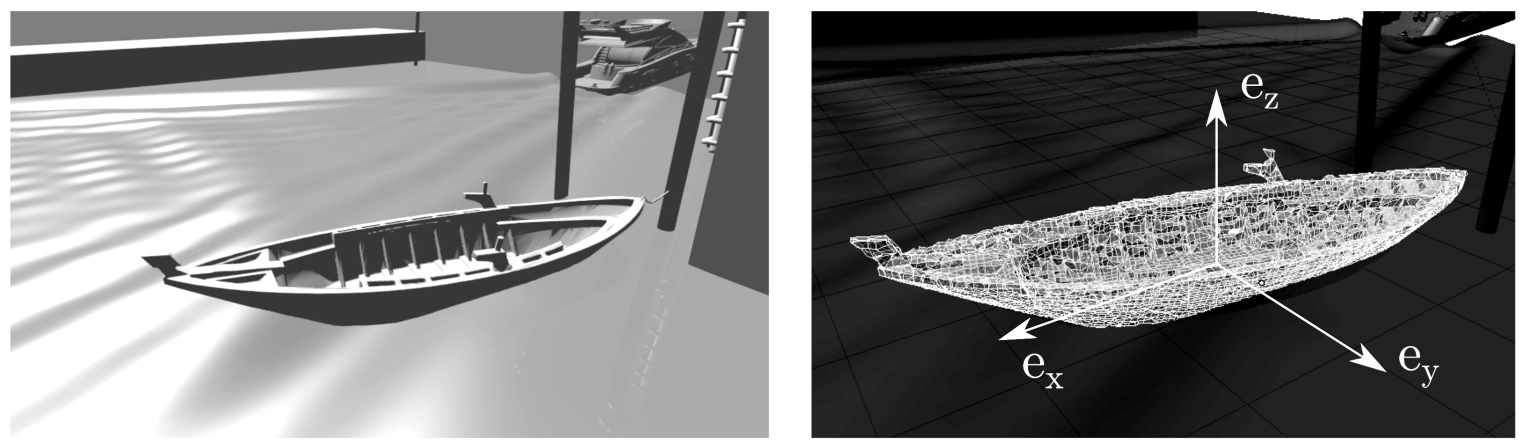
\includegraphics[width=\linewidth]{Mines_2020_coque}
\caption{Maillage de la gondole}
\end{center}
\end{figure}
%-------------------------------------------------------------------------------

Seul le mouvement de translation verticale (selon la direction verticale $\vec e_z$) est étudié.

On s’intéresse ici au maillage qui constitue la coque extérieure de la gondole. Certaines facettes sont émergées (i.e. leur barycentre est en dehors de l’eau), d’autres sont immergées (i.e leur barycentre est sous l’eau).

À chaque pas de temps, on suppose connue la fonction \type{hauteur(x,y)} qui, à tout point $(x,y)$ du plan d’eau, associe la hauteur des vagues par rapport au repère de la scène. Le maillage composant la coque de la gondole est défini dans une liste de facettes nommée \type{maillageG}.
%-------------------------------------------------------------------------------
%-------------------------------------------------------------------------------
\begin{Exercise}\it 
 Proposer une fonction \type{lister\_FI(M)} prenant comme argument un maillage \type{M} et renvoyant la liste des facettes immergées (i.e dont le centre de gravité est sous la surface définie par hauteur). On pourra utiliser les fonctions de la première partie.
\end{Exercise}
%-------------------------------------------------------------------------------
\begin{Answer}
\begin{lstlisting}
def lister_FI(M):
    L = []
    for facette in M:
        x, y, z = barycentre(facette)
        if z < hauteur(x, y):
            L.append(facette)
    return L
\end{lstlisting}
\end{Answer}
%-------------------------------------------------------------------------------
%-------------------------------------------------------------------------------

\medskip

Pour calculer la poussée d’Archimède s’exerçant sur la coque du bateau, on doit calculer la résultante des forces dues à la pression appliquées par l’eau sur chacune des facettes immergées.

On modélise la force appliquée par l’eau sur une facette $i$ par :
\[\overrightarrow{F_i} = - S_i\times p(G_i)\vec n_i\]

\begin{itemize}
    \item $S_i$ est l'aire de la facette,
    \item $\vec n_i$ est vecteur normal sortant de la coque,
    \item $p(G_i)$ est la pression hydrostatique de l’eau sur la facette en son barycentre $G_i$.
\end{itemize}

Le théorème de Pascal détermine la pression de l’eau d’un point $G$ en fonction de sa profondeur par rapport à la surface :
\[p(x_G ,y_G ,z_G) = \rho \cdot g \cdot \bigl( \type{hauteur}(x_G ,y_G) - z_g\bigr)\]
\begin{itemize}
    \item $\rho$ est masse volumique de l’eau ($\sim 1000$),
    \item $g$ est l'accélération de la pesanteur (ici : $g \sim 9,81$).
\end{itemize}

%-------------------------------------------------------------------------------
%-------------------------------------------------------------------------------
\begin{Exercise}\it 
Proposer une fonction \type{force\_facette(F)} prenant en argument une facette et renvoyant le vecteur force appliqué par l’eau sur cette facette. 
\end{Exercise}
%-------------------------------------------------------------------------------
\begin{Answer}
\begin{lstlisting}
def force_facette(F):
    S = aire(F)
    n = normale(F)
    x, y, z = barycentre(F)
    p = rho*g*(hauteur(x,y) - z)
    return -S*p*n
\end{lstlisting}
\end{Answer}
%-------------------------------------------------------------------------------
%-------------------------------------------------------------------------------
On pourra utiliser les fonctions définies précédemment et on supposera que les sommets sont donnés dans les facettes dans un ordre tel que le vecteur normal calculé est sortant.


\medskip
La force résultante sur toute la coque s’exprime par la somme de toutes les forces appliquées sur chaque facette immergée.
%-------------------------------------------------------------------------------
%-------------------------------------------------------------------------------
\begin{Exercise}\it 
Définir la fonction \type{resultante(L)} prenant comme argument une liste \type{L} de facettes (supposées immergées), renvoyant la somme des forces, sur l’axe $\vec e_z$ de l’eau, appliquée sur l’ensemble des surfaces.
\end{Exercise}
%-------------------------------------------------------------------------------
\begin{Answer}
\begin{lstlisting}
def resultante(L):
    res = 0.
    for F in L:
        res = res + force_facette(F)[2]
    return res
\end{lstlisting}
\end{Answer}
%-------------------------------------------------------------------------------
%-------------------------------------------------------------------------------
\medskip

 On cherche à optimiser l’efficacité de la fonction \type{resultante} qui devra être utilisée intensément pour réaliser un grand nombre d’images. On remarque que la taille des facettes n’est pas homogène : la coque est composée de grandes facettes et de petites facettes. Les petites facettes représentent souvent des détails d’intérêt graphique n’apportant qu’une très faible contribution à la résultante  des forces hydrostatiques.
 
Ainsi, une étude montre que la moitié des facettes représente à elle seule 99\% de la surface totale  de la coque. Pour alléger le processus, on trier les facettes par aire décroissante, afin de n’appliquer les calculs de la poussée d’Archimède qu'à la moitié d’entre elles (les plus grandes). La fonction de tri est supposée donnée sous le nom \type{trier\_facettes}.
%-------------------------------------------------------------------------------
%-------------------------------------------------------------------------------
\begin{Exercise}\it 
 Affecter à une nouvelle variable \type{grandesFacettes} la liste des facettes de privée de la moitié des facettes les plus petites (en cas de nombre impair d’éléments, on inclura la facette médiane).
\end{Exercise}
%-------------------------------------------------------------------------------
\begin{Answer}
\begin{lstlisting}
n = len((maillageG)
p = (n + 1)//2
facettes_triees = trier_facettes(maillageG)
grandesFacettes = facettes_triees[ : p]
\end{lstlisting}
\end{Answer}
%-------------------------------------------------------------------------------
%-------------------------------------------------------------------------------

\medskip

La gondole est attachée à un repère local dont l’origine est son centre de gravité (de coordonnées $(x_G ,y_G ,z_G)$ et de vitesse verticale notée $v$) par rapport au décor. Le principe fondamental de la dynamique en projection sur l’axe vertical $\vec e_z$ appliqué à la gondole énonce que 
\[\left\{\begin{matrix}
\displaystyle \frac{\d v}{\d t} &=&\frac 1m\times F_g - g\\ 
\displaystyle \frac{\d z_G}{\d t} &=& v\\ 
\end{matrix}\right.\]
\begin{itemize}
    \item $m$ est la masse de la gondole,
    \item $F_g$ est la résultante des forces appliquées par l’eau sur la gondole (renvoyée par la fonction \type{resultante}, vue précédemment).
\end{itemize}
La position initiale de la gondole est $z_{G,0} = 0$. Sa vitesse verticale initiale est $v_0 = 0$.

On souhaite estimer le mouvement par la méthode d’Euler. Pour ce faire, on utilise la fonction \type{nouvelle\_hauteur} avant d’afficher chaque nouvelle image. Cette fonction a pour but de recalculer la hauteur (et la vitesse) de la gondole pour un nouveau pas de temps. Elle prend trois arguments :

\begin{itemize}
\item \type{posG} contiendra le vecteur position actuel du centre de gravité de la gondole au moment de
l’appel,
\item \type{vitG} contiendra le vecteur vitesse actuel de ce même point au moment de l’appel,
\item \type{mailG}  ontiendra la liste des grandes facettes de la gondole (privée des petites, au sens de la
question précédente), au moment de l’appel.
\end{itemize}
\begin{lstlisting}
def nouvelle_hauteur(posG, vitG, mailG):
    dt = 1/25 # Pas de temps correspondant à une image du film
    facettes_immergees = lister_FI(mailG)
    posG = posG + .......... # à compléter
    vitG = vitG + .......... # à compléter
    return posG, vitG
\end{lstlisting}
%-------------------------------------------------------------------------------
%-------------------------------------------------------------------------------
\begin{Exercise}\it 
Compléter les lignes 4 et 5 du code précédent conformément à la méthode d’Euler.
\end{Exercise}
%-------------------------------------------------------------------------------
\begin{Answer}
\begin{lstlisting}
def nouvelle_hauteur(posG, vitG, mailG):
    dt = 1/25 
    facettes_immergees = lister_FI(mailG)
    posG = posG + dt*vitG 
    vitG = vitG + dt*(resultante(facettes_immergees)/m - g)
    return posG, vitG
\end{lstlisting}
\end{Answer}
%-------------------------------------------------------------------------------
%-------------------------------------------------------------------------------



% code Python
% 1
% 2
% 3
% 4
% 5
% 6
% def nouvelle_hauteur ( posG , vitG , mailG ):
% dt =1.0/25.0 # Pas de temps correspondant à une image du film.
% facettes_immergees = lister_FI ( mailG )
% posG = posG + ..........
% # à compléter
% vitG = vitG + ...........
% # à compléter
% return posG , vitG
% o Q27 – 
% FIN DE L’ÉPREUVE
% 12